\documentclass[11pt,a4paper,oneside]{article}

\usepackage[T2A]{fontenc}
\usepackage[utf8]{inputenc}
\usepackage[english,russian]{babel}
\usepackage[russian]{olymp}
\usepackage{graphics}
\usepackage{wrapfig}
\usepackage{amsmath}
\usepackage{amssymb}
\usepackage{epigraph}
\usepackage{graphicx}

\contest{ACM ICPC Kyrgyzstan Subregional 2015}{Бишкек}{1 ноября 2015 года}    

\binoppenalty=10000

\relpenalty=10000
\exhyphenpenalty=10000

\renewcommand{\t}{\texttt}

\createsection{\Note}{Примечание}

\renewcommand{\defaultmemorylimit}{256 мегабайт}

\begin{document}

\begin{problem}{Точки на окружности}{1 секунда}{32 мегабайта}

\noindent
На окружности расположены $N$ точек ($N>2$), пронумерованных от $0$ до $N-1$ по часовой стрелке. 
Изначально точки незакрашены.
Нурбек выбирает число $2 \le K < N$ и начинает закрашивать каждую $K$-ую точку на окружности в красный цвет.
Так, на первом шаге Нурбек закрашивает точку с номером $K$, на втором - $(2K)~mod~N$, на третьем  - $(3K)~mod~N$, на $i$-том - $(iK)~mod~N$, и.т.д. Нурбек заканчивает раскраску на таком шаге $j$, что точка с номером $(jK)~mod~N$ уже была закрашена на одном из предыдущих шагов.

\medskip\noindent
Например, при $N=6$ и $K=4$, на первом шаге будет закрашена точка с номером 4, на втором - точка с номером  2 (т.к. $(4\cdot 2)~mod~6$ = $8~mod~6$ = $2$), на третьем - точка с номером 0 (т.к. $(4 \cdot 3)~mod~6$ = $12~mod~6$ = $0$). На четвертом шаге Нурбек увидит, что точка с номером 4 уже закрашена, и остановится.
Закрашенные точки после каждого шага показаны на Рис.1. 





\begin{figure}[ht]
\centering
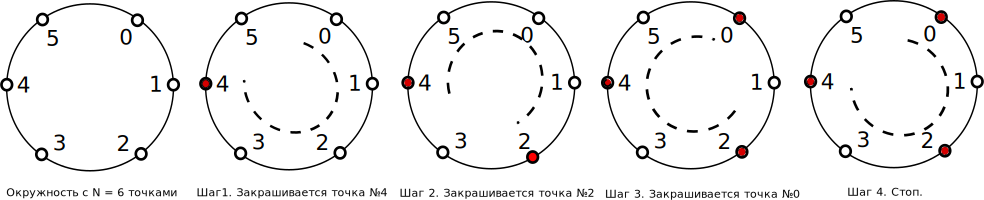
\includegraphics[width=0.8\textwidth]{drawing-1.pdf}
\caption{ Точки на окружности. $N=6$, $K = 4$}
\end{figure}

\noindent
Задача Нурбека - закрасить все точки. Найдите наименьшее $2 \le K < N$ такое, что все точки будут закрашены (то есть, Нурбек остановится на $N+1$ первом шаге после закраски всех $N$ точек).

\InputFile

\noindent
В первой и единственной строке входных данных записано число $3 \le N \le 2 \cdot 10^9$ -  количество точек.


\OutputFile

\noindent
Выведите  наименьшее $K$ ($2 \le K < N$ ), такое, что все точки будут закрашены (то есть, Нурбек остановится на $N+1$ первом шаге после закраски всех $N$ точек).


\Examples
\begin{example}%
\exmp{
6
}{
5
}%
\exmp{
3
}{
2
}%
\end{example}

\vspace{1cm}



\hfill \textit{Автор задачи: Евгений Балай}


\end{problem}


\end{document}
%%% Local Variables:
%%% mode: latex
%%% TeX-master: t
%%% End:
